\documentclass[10pt,a4paper]{article}

\usepackage[margin=1.7cm]{geometry}
\usepackage{booktabs}
\usepackage{tabularx}
\usepackage{graphicx}
\usepackage{hyperref}
\usepackage{xcolor}
\usepackage{tikz}
\usetikzlibrary{arrows.meta,positioning,calc}
\usepackage{enumitem}
\usepackage{caption}
\usepackage{fancyhdr}

\hypersetup{colorlinks=true,linkcolor=blue!50!black,urlcolor=blue!60!black}
\captionsetup{font=small,labelfont=bf}
\setlist{nosep,leftmargin=*}
\pagestyle{fancy}
\fancyhf{}
\fancyhead[L]{\small Raspberry~Pi~5 OP-TEE}
\fancyhead[R]{\small Final Report \& User Manual}
\fancyfoot[C]{\thepage}
\renewcommand{\headrulewidth}{0.3pt}

\newcommand{\cmd}[1]{\texttt{\detokenize{#1}}}

\title{\textbf{Raspberry Pi~5 Real OP-TEE Deployment}\\[0.25em]
\large Engineering Report, Failure Log, and User Manual}
\author{pi5-optee project}
\date{August 2026}

\begin{document}
\maketitle
\vspace{-1.1em}
\begin{abstract}
\noindent
This document is the final report for bringing \textbf{real OP-TEE} to a
Raspberry~Pi~5. It covers architecture and memory layout, a short chronology of
every major failure and retry, the hardened LAN build/deploy/test scripts,
validation results (\cmd{xtest}), and a user manual for rebuild and redeploy.
Page budget: at most 10 pages.
\end{abstract}

%% --------------------------------------------------------------------
\section{Introduction and Goals}
The goal was a Trusted Execution Environment on Pi~5 that is usable for
real workloads and regression testing---not QEMU-only OP-TEE. That required:
(1)~an embedded BL31+OP-TEE armstub loaded by the VPU; (2)~correct
\cmd{kernel_address} so Linux does not destroy the stub; (3)~a custom kernel
with \cmd{CONFIG_TEE}/\cmd{CONFIG_OPTEE}; (4)~userspace
(\cmd{tee-supplicant}, libteec, TAs, \cmd{xtest}); (5)~LAN automation that does
not destroy Wi‑Fi configuration.

\begin{table}[ht]
\centering
\caption{Final software stack (validated on Pi~5).}
\label{tab:stack}
\begin{tabular}{@{}llp{5.8cm}@{}}
\toprule
\textbf{Layer} & \textbf{Component} & \textbf{Role} \\
\midrule
Firmware & \cmd{armstub8-2712-optee.bin} (1\,MiB) & BL31 + tee-raw embedded \\
Secure OS & OP-TEE OS (plat-rpi5), CFG\_DT=y & BL32 in TZDRAM; DT patched at boot \\
Kernel & \cmd{kernel_2712-optee.img} & TEE/OPTEE drivers $\rightarrow$ \cmd{/dev/tee*} \\
Userspace & tee-supplicant, libteec, xtest, TAs & RPC + regression suite \\
Host & Shell scripts under \cmd{~/pi5-optee} & Build, LAN deploy, test, recover \\
\bottomrule
\end{tabular}
\end{table}

%% --------------------------------------------------------------------
\section{Architecture}
Figure~\ref{fig:boot} shows the boot handoff. Figure~\ref{fig:mem} shows why
\cmd{kernel_address=0x200000} is mandatory: the embedded OP-TEE image occupies
\texttt{[0x80000,0x100000)} inside the armstub until BL31 copies it to TZDRAM.

\begin{figure}[ht]
\centering
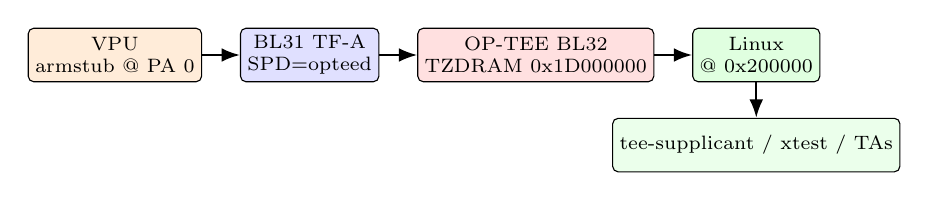
\begin{tikzpicture}[
  node distance=0.32cm and 0.48cm,
  box/.style={draw,rounded corners=2pt,align=center,font=\scriptsize,
              minimum height=0.68cm,inner sep=2.5pt},
  arr/.style={-{Latex},thick}
]
\node[box,fill=orange!15] (vpu) {VPU\\armstub @ PA 0};
\node[box,fill=blue!12,right=of vpu] (bl31) {BL31 TF-A\\SPD=opteed};
\node[box,fill=red!12,right=of bl31] (tee) {OP-TEE BL32\\TZDRAM 0x1D000000};
\node[box,fill=green!12,right=of tee] (linux) {Linux\\@ 0x200000};
\node[box,fill=green!8,below=0.45cm of linux] (ree) {tee-supplicant / xtest / TAs};
\draw[arr] (vpu)--(bl31);
\draw[arr] (bl31)--(tee);
\draw[arr] (tee)--(linux);
\draw[arr] (linux)--(ree);
\end{tikzpicture}
\caption{Pi~5 OP-TEE boot chain.}
\label{fig:boot}
\end{figure}

\begin{figure}[ht]
\centering
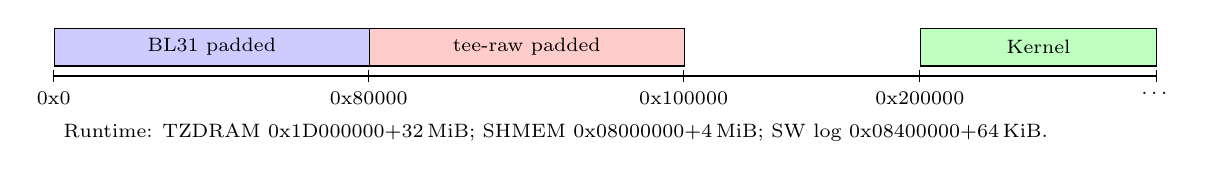
\begin{tikzpicture}[font=\scriptsize,bar/.style={draw,minimum height=0.48cm,align=center}]
\draw[thick] (0,0)--(14,0);
\foreach \x/\lab in {0/0x0,4/0x80000,8/0x100000,11/0x200000,14/\ldots} {
  \draw (\x,0.08)--(\x,-0.08) node[below] {\lab};
}
\node[bar,fill=blue!20,minimum width=4cm,anchor=south west] at (0,0.12) {BL31 padded};
\node[bar,fill=red!20,minimum width=4cm,anchor=south west] at (4,0.12) {tee-raw padded};
\node[bar,fill=green!25,minimum width=3cm,anchor=south west] at (11,0.12) {Kernel};
\node[anchor=west] at (0,-0.72)
  {Runtime: TZDRAM 0x1D000000+32\,MiB; SHMEM 0x08000000+4\,MiB; SW log 0x08400000+64\,KiB.};
\end{tikzpicture}
\caption{Armstub physical layout and kernel load address.}
\label{fig:mem}
\end{figure}

\begin{table}[ht]
\centering
\caption{Required \cmd{/boot/firmware/config.txt} keys.}
\label{tab:config}
\begin{tabular}{@{}llp{5.5cm}@{}}
\toprule
\textbf{Key} & \textbf{Value} & \textbf{Notes} \\
\midrule
\cmd{armstub} & \cmd{armstub8-2712-optee.bin} & Never plain \cmd{bl31.bin} alone \\
\cmd{kernel_address} & \cmd{0x200000} & Avoids overwrite of embed region \\
\cmd{arm_64bit} & \cmd{1} & 64-bit kernel \\
\cmd{dtoverlay=optee-rpi5} & \emph{disabled} & Redundant with CFG\_DT=y \\
\bottomrule
\end{tabular}
\end{table}

%% --------------------------------------------------------------------
\section{Chronology: Failures and Tries}
Table~\ref{tab:failures} compresses the engineering history (24--29~Aug~2026).
Early firmware experiments repeatedly left the board unreachable; the team
initially attributed this to ``Wi‑Fi deleted.'' Investigation showed boot hangs
from incorrect stubs/addresses, while NetworkManager profiles usually remained.
Ethernet became the preferred path for first OP-TEE reboots. A fresh Raspberry~Pi
Imager image (29~Aug) plus LAN deploy scripts produced a clean validation run.

\begin{table}[ht]
\centering
\caption{Failure log (short) and corrective try.}
\label{tab:failures}
\footnotesize
\begin{tabularx}{\textwidth}{@{}c>{\raggedright\arraybackslash}p{2.9cm}
  >{\raggedright\arraybackslash}X>{\raggedright\arraybackslash}p{3.2cm}@{}}
\toprule
\textbf{\#} & \textbf{Try / symptom} & \textbf{Cause} & \textbf{Fix} \\
\midrule
1 & Believed 32-bit OS mandatory & Doc confusion & 64-bit Bookworm is correct \\
2 & SSH/Wi‑Fi ``lost'' after stub & Boot hang, not wiped NM & Ethernet; boot FAT recovery; scripts never rewrite Wi‑Fi \\
3 & Used plain BL31 as armstub & No embedded BL32 & 1\,MiB embedded armstub only \\
4 & Kernel crushed OP-TEE & Default load @ 0x80000 & \cmd{kernel_address=0x200000} \\
5 & Bad reserved-memory / probe & Overlay + CFG\_DT=y clash & Comment out \cmd{dtoverlay=optee-rpi5} \\
6 & Blank \cmd{armstub=} remotely & \cmd{sudo -S} stole stdin & Write keys via \cmd{bash -c} args \\
7 & \cmd{ETXTBSY} on supplicant & File busy while running & Stop/kill before copy \\
8 & Modules under nested \cmd{KREL} & \cmd{scp -r} nesting & \cmd{rsync}; skip dangling \cmd{build} link \\
9 & Default host was Wi‑Fi IP & Mixed script defaults & Default to Ethernet LAN IP \\
10 & No \cmd{/dev/tee*} & Stock kernel lacks TEE & Custom OP-TEE kernel + modules \\
11 & Imager then SD vs LAN copy & Ops choice & LAN deploy after Imager \\
12 & \cmd{xtest} 1033 failed & Missing \cmd{*.plugin} & Install plugin; stage in build \\
\bottomrule
\end{tabularx}
\end{table}

\begin{figure}[ht]
\centering
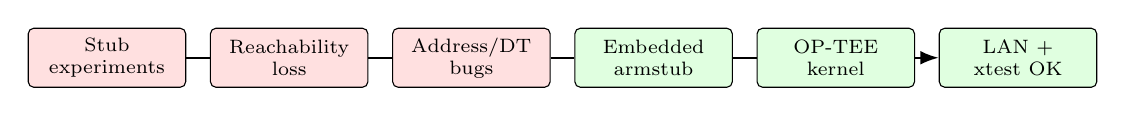
\begin{tikzpicture}[
  font=\scriptsize,
  stage/.style={draw,rounded corners=2pt,align=center,minimum width=2.0cm,minimum height=0.75cm},
  bad/.style={stage,fill=red!12}, good/.style={stage,fill=green!12},
  arr/.style={-{Latex},thick}]
\node[bad] (a) {Stub\\experiments};
\node[bad,right=0.3cm of a] (b) {Reachability\\loss};
\node[bad,right=0.3cm of b] (c) {Address/DT\\bugs};
\node[good,right=0.3cm of c] (d) {Embedded\\armstub};
\node[good,right=0.3cm of d] (e) {OP-TEE\\kernel};
\node[good,right=0.3cm of e] (f) {LAN +\\xtest OK};
\draw[arr] (a)--(b)--(c)--(d)--(e)--(f);
\end{tikzpicture}
\caption{From failed tries to validated stack.}
\label{fig:timeline}
\end{figure}

%% --------------------------------------------------------------------
\section{Tooling: Artifacts and Scripts}
Artifacts land in \cmd{artifacts/rpi5-optee/} (armstub, tee*.bin, kernel image,
modules staging, rootfs overlay with xtest/TAs/plugin). Figure~\ref{fig:pipeline}
shows the LAN pipeline.

\begin{figure}[ht]
\centering
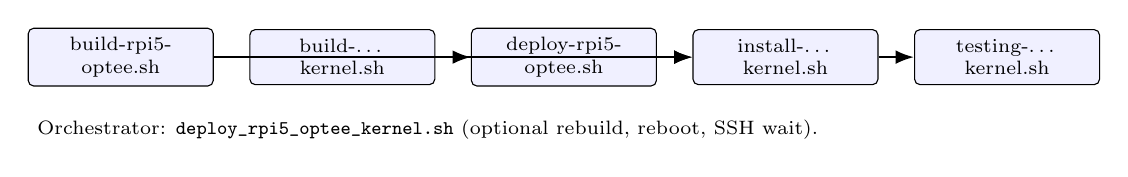
\begin{tikzpicture}[
  font=\scriptsize,
  box/.style={draw,rounded corners=2pt,align=center,fill=blue!6,
              minimum width=2.35cm,minimum height=0.7cm},
  arr/.style={-{Latex},thick}]
\node[box] (b1) {build-rpi5-\\optee.sh};
\node[box,right=0.45cm of b1] (b2) {build-\ldots\\kernel.sh};
\node[box,right=0.45cm of b2] (d1) {deploy-rpi5-\\optee.sh};
\node[box,right=0.45cm of d1] (d2) {install-\ldots\\kernel.sh};
\node[box,right=0.45cm of d2] (t1) {testing-\ldots\\kernel.sh};
\draw[arr] (b1)--(d1);
\draw[arr] (b2)--(d2);
\draw[arr] (d1)--(d2);
\draw[arr] (d2)--(t1);
\node[font=\scriptsize,anchor=west] at ($(b1.south west)+(0,-0.55)$)
  {Orchestrator: \cmd{deploy_rpi5_optee_kernel.sh} (optional rebuild, reboot, SSH wait).};
\end{tikzpicture}
\caption{Build $\rightarrow$ deploy $\rightarrow$ test pipeline.}
\label{fig:pipeline}
\end{figure}

\begin{table}[ht]
\centering
\caption{Primary scripts.}
\label{tab:scripts}
\begin{tabular}{@{}lp{8.4cm}@{}}
\toprule
\textbf{Script} & \textbf{Purpose} \\
\midrule
\cmd{build-rpi5-optee.sh} & TF-A, OP-TEE OS, armstub, rootfs overlay (+ plugin) \\
\cmd{build-rpi5-optee-kernel.sh} & \cmd{Image.gz} + modules with OP-TEE fragment \\
\cmd{deploy-rpi5-optee.sh} & SCP armstub/userspace; safe \cmd{config.txt} updates \\
\cmd{install-rpi5-optee-kernel.sh} & Install kernel + modules; password-aware reboot \\
\cmd{deploy_rpi5_optee_kernel.sh} & One-shot orchestration over LAN \\
\cmd{testing_rpi5_optee_kernel.sh} & Smoke + \cmd{xtest} \\
\cmd{monitoring_rpi5_optee_secure_world.sh} & NW command with SW log follow \\
\cmd{recover-boot-wifi.sh} & Offline boot FAT recovery helpers \\
\bottomrule
\end{tabular}
\end{table}

%% --------------------------------------------------------------------
\section{Validation Results}
Target after Imager + LAN deploy: \cmd{skmitra@192.168.0.107}.

\begin{itemize}
  \item Kernel \cmd{6.18.46-v8-16k+}; \cmd{/dev/tee0}, \cmd{/dev/teepriv0} present.
  \item \cmd{tee-supplicant} active; eth0 connected.
  \item \cmd{config.txt}: correct \cmd{armstub} and \cmd{kernel_address}.
  \item \cmd{xtest -l 0}: 114 cases; one initial failure (1033) due to missing
        tee-supplicant plugin; after install, 1033 OK.
  \item Expected skips: pseudo-TA / fTPM / PAuth / MTE / some PTA cases.
\end{itemize}

\begin{table}[ht]
\centering
\caption{\cmd{xtest -l 0} summary.}
\label{tab:xtest}
\begin{tabular}{@{}lr@{}}
\toprule
\textbf{Metric} & \textbf{Value} \\
\midrule
Regression cases & 114 \\
Failures after plugin fix & 0 \\
Initial sole failure & regression\_1033 (plugin not found) \\
\bottomrule
\end{tabular}
\end{table}

%% --------------------------------------------------------------------
\section{User Manual}
\subsection{Prerequisites}
Build host (Debian/Ubuntu) with packages for TF-A/OP-TEE and kernel builds
(\cmd{bc}, \cmd{bison}, \cmd{flex}, \cmd{libssl-dev}, \ldots). Pi~5 on
\textbf{64-bit} Bookworm with SSH. Prefer Ethernet for first OP-TEE reboots.
Set \cmd{export PI_SUDO_PASSWORD='...'} (or \cmd{SSHPASS}); do not hardcode secrets.

\subsection{Build}
\begin{verbatim}
cd ~/pi5-optee
OPTEE_MAX_LOG=1 ./build-rpi5-optee.sh
./build-rpi5-optee-kernel.sh   # if kernel not built by the above
\end{verbatim}
Sanity checks: armstub size $=1048576$; OP-TEE region matches \cmd{tee-raw.bin}
at offset \cmd{0x80000}; overlay contains \cmd{xtest}, TAs, and
\cmd{usr/lib/tee-supplicant/plugins/*.plugin}.

\subsection{Deploy over LAN}
\begin{verbatim}
export PI_SUDO_PASSWORD='...'
./deploy_rpi5_optee_kernel.sh --skip-build --skip-kernel-config-fetch \
    USER@PI_LAN_IP
\end{verbatim}
Without \cmd{--skip-build}, the orchestrator rebuilds then deploys. Reboot is
performed with password-aware sudo. Wait for SSH (Ethernet and known Wi‑Fi IPs
are both probed when defaults match the project hosts).

\subsection{Test and monitor}
\begin{verbatim}
./testing_rpi5_optee_kernel.sh USER@PI_LAN_IP
./monitoring_rpi5_optee_secure_world.sh USER@PI_LAN_IP -- xtest -l 0
# On device: sudo optee-sw-log -f
\end{verbatim}

\subsection{Recovery}
If SSH dies after enabling the stub, treat it as a \textbf{boot hang}:
\begin{enumerate}
  \item Connect Ethernet; try the LAN address.
  \item Mount the boot FAT elsewhere; disable \cmd{armstub=} or rename the
        stub; restore from \cmd{/boot/firmware.file-backups/}.
  \item Run \cmd{recover-boot-wifi.sh} on the SD boot partition.
\end{enumerate}

\subsection{Checklists and troubleshooting}
\begin{table}[ht]
\centering
\caption{Pre-reboot checklist.}
\label{tab:checklist}
\begin{tabular}{@{}lp{7.2cm}@{}}
\toprule
\textbf{Item} & \textbf{OK criterion} \\
\midrule
Armstub & 1\,MiB; embeds current \cmd{tee-raw} \\
\cmd{config.txt} & Correct \cmd{armstub} + \cmd{kernel_address=0x200000} \\
DT overlay & \cmd{optee-rpi5} disabled \\
Kernel/modules & Matching OP-TEE Image and \cmd{/lib/modules/$KREL} \\
Plugin & Present under tee-supplicant plugins dir \\
Network & Ethernet path verified before reboot \\
\bottomrule
\end{tabular}
\end{table}

\begin{table}[ht]
\centering
\caption{Troubleshooting quick reference.}
\label{tab:trouble}
\begin{tabular}{@{}lp{7.6cm}@{}}
\toprule
\textbf{Symptom} & \textbf{Likely action} \\
\midrule
No \cmd{/dev/tee*} & Install OP-TEE kernel; confirm dmesg OP-TEE probe \\
Boot then silence & Revert armstub; check \cmd{kernel_address} \\
xtest 1033 fails & Install \cmd{*.plugin}; restart tee-supplicant \\
Modules missing deps & Re-run install with \cmd{rsync} (not nested scp) \\
ETXTBSY on copy & \cmd{systemctl stop tee-supplicant} then retry \\
\bottomrule
\end{tabular}
\end{table}

%% --------------------------------------------------------------------
\section{Lessons Learned}
\begin{itemize}
  \item Pi~5 needs an \textbf{embedded} armstub and a non-default kernel load
        address; TF-A alone is not enough.
  \item Reachability loss after OP-TEE experiments was usually a \textbf{bad boot},
        not deleted Wi‑Fi---automation must never rewrite NM/netplan casually.
  \item Small automation defects (\cmd{sudo -S} stdin, \cmd{scp -r} nesting) can
        silently blank firmware keys or break module trees.
  \item Stock Raspberry~Pi kernels omit TEE drivers; custom OP-TEE kernels are
        required for \cmd{/dev/tee*} and meaningful \cmd{xtest} coverage.
\end{itemize}

\section{Appendix: Runtime Addresses}
\begin{table}[ht]
\centering
\caption{Runtime regions used by this port (see \cmd{MEMORY-LAYOUT.txt}).}
\label{tab:runtime}
\begin{tabular}{@{}llp{5.2cm}@{}}
\toprule
\textbf{Region} & \textbf{Base / size} & \textbf{Purpose} \\
\midrule
TZDRAM / BL32 & 0x1D000000 / 32\,MiB & OP-TEE secure DRAM \\
Shared memory & 0x08000000 / 4\,MiB & NW$\leftrightarrow$SW buffers \\
SW log ring & 0x08400000 / 64\,KiB & \cmd{optee-sw-log} over SSH \\
Kernel load & 0x200000 & Avoids armstub OP-TEE pad \\
\bottomrule
\end{tabular}
\end{table}

\noindent\textbf{Handoff note:} BL32 entry uses opteed conventions
(\cmd{arg0=MODE_RW_64}, DTB PA in \cmd{arg3}). Do not enable the legacy
device-tree overlay when CFG\_DT=y is set.

\section*{Document control}
Repository: \cmd{pi5-optee}. Sources: scripts, \cmd{MEMORY-LAYOUT.txt}, and
sessions 24--29~Aug~2026. Compile: \cmd{tectonic rpi5-optee-manual.tex} or
\cmd{pdflatex} twice. Limit: $\leq$\,10 pages.

\end{document}
